\chapter{Existenz von Nash-Gleichgewichten}%
\label{cha:Existenz von Nash-Gleichgewichten}

Spieler $i = 1, \ldots, N$ lösen
\[
	\min\limits_{x^{i}} f_{i}(x^{i}, x^{-i}) \quad \text{ udN } x^{i} \in X_{i}
.\] 

Gängige Annahmen sind
\begin{itemize}
	\item $X \in \R^{n}$ nichtleer, konvexm abgeschlossen, gelegentlich kompakt
	\item $f \colon \R^{n} \rightarrow \R $ stetig (differenzierbar), konvex bezüglich $x^{i}$
\end{itemize}

Fall $n=1$: Optimierungsproblem
\[
	\min\limits_{x}f(x) \quad \text{ udN } x \in X
.\] 

\begin{definition}
\label{thm:variationsungleichung}
Sei $X \subseteq \R^{n}$ nichtleer und $F \colon X \rightarrow \R^{n} $. Dann besteht das \enter
\underline{Variationsungleichungsproblem} $\text{VIP}(X,F)$ darin, einen Punkt ${x}^{*} \in X$ zu finden sodass
\[
	F({x}^{*})^{T}(x-{x}^{*}) \geq  0 \quad \forall x \in X
.\] 
\end{definition}

\begin{lemma}
\label{thm:lemmavariation}
Für $X=\R^{n}$ und $F \colon \R^{n} \rightarrow \R^{n} $ ist VIP($X,F$) äquivalent zur Bestimmung von Lösungen von $F(x) = 0$.
\end{lemma}

\begin{proof}
\label{thm:lemmavariationbeweis}
\begin{itemize}
	\item "$\Longleftarrow$":

		Gilt $F({x}^{*})=0$ und ${x}^{*} \in \R^{n} = X$, so folgt
		\[
			F({x}^{*})^{T}(x-{x}^{*}) \geq  0 \quad \forall x \in \R^{n}
		.\] 
	\item "$\Longrightarrow$":

		Sei ${x}^{*} \in \R^{n}$ nun eine Lösung von VIP($X,F$), d.h. es gelte
		\[
			F({x}^{*})^{T}(x-{x}^{*}) \geq  0 \quad \forall x \in \R^{n}
		.\] 
		Setze nun $x = {x}^{*} - F({x}^{*})$ ein. Dann folgt
		\begin{align*}
			&F({x}^{*})^{T}(x-{x}^{*}) \geq  0 \\
			\implies
			&F({x}^{*})^{T}({x}^{*}-F({x}^{*})-{x}^{*}) \geq  0 \\
			\implies
			&-\norm{F({x}^{*})} _{2}^2 \geq  0 \\
			\implies
			&F({x}^{*}) = 0
		\end{align*}
\end{itemize}
\end{proof}

\begin{definition}
\label{thm:komplementaritätsproblem}
Sei $F \colon \R^{n} \rightarrow \R^{n} $. Dann besteht das \underline{Komplementaritätsproblem}  NCP($F$) darin, einen Punkt ${x}^{*} \in \R^{n}$ zu finden mit $\forall i=1, \ldots, n$ gilt
\[
	x_{i}^{*} \geq  0,\quad F_{i}({x}^{*}) \geq 0, \qquad x_{i}^{*}F_{i}({x}^{*}) = 0
.\] 
Ist $F$ linear, d.h. $F(x) = Mx + q$, so spricht man von einem\\ \underline{linearen Komplementaritätsproblem} LCP($q,M$).
\end{definition}

\begin{beisp}
\label{thm:komplementaritätsproblembeispiel}
	Betrachte das quadratische Problem
	\[
	\min\limits_{x}\frac{1}{2} x^{T} Q x + q^{T}x \quad \text{ udN } Ax \leq  b, x \geq  0
	.\] 
	zugehöriges KKT-System
	\begin{align*}
		0 &= Qx + q + A^{T} \lambda - \gamma  \\
		Ax &\leq  b \\
		\lambda &\geq  0 \\
		(Ax-b)_{i}\lambda _{i} &= 0 \quad \forall i \\
		x &\geq  0 \\
		\gamma &\geq  0 \\
		x_{i}\gamma_{i} &= 0 \quad \forall i
	\end{align*}
	\begin{align*}
		\iff\qquad\qquad\qquad\qquad\qquad &\\
	\begin{pmatrix}
	x \\
	\lambda 
\end{pmatrix} &\geq 0 \\
\underbrace{\begin{pmatrix}
		Q & A^{T} \\ A & 0
\end{pmatrix}
}_{=:M} \begin{pmatrix}
x \\ \lambda 
\end{pmatrix}
+ \underbrace{\begin{pmatrix}
q \\ b
\end{pmatrix}
}_{=:c} 
&\geq 0
	\end{align*}
	bzw. kürzer
	\begin{align*}
		\iff\qquad\qquad\qquad\qquad\qquad &\\
	\begin{pmatrix}
	x \\
	\lambda 
\end{pmatrix} &\geq 0 \\
\begin{pmatrix}
x \\ \lambda 
\end{pmatrix}
_{i}\left( M \begin{pmatrix}
x \\ \lambda 
\end{pmatrix}
	+ c \right) _{i} &\geq  0
	\end{align*}
\end{beisp}

\begin{lemma}
	%\label{thm:}
	Für $X = \R^{n}$ und $F \colon \R^{n} \rightarrow \R^{n} $ ist VIP($X,F$) äquivalent zu NCP($F$)
\end{lemma}

\begin{proof}
	%\label{thm:}
	\begin{itemize}
		\item "$\Longleftarrow$":

			Sei ${x}^{*}$ eine Lösung von NCP($F$), d.h. ${x}^{*}\geq 0, F({x}^{*}) \geq  0$ und $\forall i =1, \ldots, n: \quad {x}^{*}_{i} F_{i}({x}^{*}) = 0$.

			Dann gilt ${x}^{*} \in \R^{n}_{+}=X$ und für alle $x \in X$ gilt
			\[
				F({x}^{*})^{T}(x-{x}^{*}) = \sum_{i=1}^{n}{\underbrace{F_{i}({x}^{*})}_{\geq 0} \underbrace{x_{i}}_{\geq 0}} - \underbrace{F({x}^{*})^{T}{x}^{*}}_{=0} \geq 0
			.\] 
			\[
				\implies {x}^{*} \text{ löst VIP}(X,F) 
			.\] 
		\item "$\Longrightarrow$":

			Sei ${x}^{*}$ eine Lösung von VIP($X,F$). Dann gilt ${x}^{*} \in X$, d.h. ${x}^{*}\geq 0$.

			Für alle $i$ mit ${x}^{*}_{i}=0$ gilt ${x}^{*}_{i}F_{i}({x}^{*})=0$. Sei ${x}^{*}_{i}>0$, dann gilt für $x = {x}^{*} \pm {x}^{*}_{i}e_{i}\geq 0$
			\[
				F({x}^{*})^{T}(x-{x}^{*}) = \pm F_{i}({x}^{*}){x}^{*}_{i}\geq 0 \implies
				\begin{array}{r}
					F_{i}({x}^{*})\geq 0 \\
					F_{i}({x}^{*})\leq 0
				\end{array}
				\implies F_{i}({x}^{*}) = 0
			.\] 
			Also gilt in jedem Fall
			\[
				F_{i}({x}^{*})\geq  0
			.\] 
	\end{itemize}
\end{proof}

\begin{beisp}
%\label{thm:}
	\[
		\min\limits_{x}f(x) \quad \text{ udN } g(x)\leq  0, h(x) = 0
	.\] 
	KKT-Bedingungen:
	\begin{align*}
		\nabla f({x}) + \nabla g({x}) \lambda  + \nabla h({x})\mu &= 0 \\
		h({x}) &= 0 \\
		g({x}) &\leq 0 \\
		\lambda &\geq  0 \\
		g({x})\lambda _{i} &= 0 \quad \forall i = 1, \ldots, m
	\end{align*}
	Definiere
	\begin{align*}
		z &= \begin{pmatrix}
	x \\ \lambda \\ \mu 
	\end{pmatrix}
	\\
			Z &= \R^{n} \times \R^{m}_{+} \times \R^{p}
	\\
			F(x, \lambda ,\mu ) &= \begin{pmatrix}
		\nabla f(x) + \nabla g(x)\lambda  + \nabla h(x)\mu  \\
		-g(x) \\
		h(x)
	\end{pmatrix}
	\end{align*}
	$\implies$ KKT äquivalent tu VIP($Z,F$).
\end{beisp}

Betrachte ein Optimierungsproblem
\[
	\min\limits_{x}f(x) \quad \text{ udN }x \in X
\] 
mit $X \subseteq \R^{n}$ nichtleer, abgeschlossen, konvex und $f \colon X \rightarrow \R $ stetig diffbar (auf offener Obermenge von X). Dann besagt das Minimum-Prinzip:
\begin{enumerate}[label=(\alph{enumi})]
	\item Ist ${x}^{*}$ ein lokales Minimum von $f$ auf $X$, dann gilt 
		\[
			\nabla  f({x}^{*})^{T}(x-{x}^{*}) \geq  0 \quad \forall x \in X
		,\] 
		d.h. ${x}^{*}$ löst VIP($X,\nabla f$).
	\item Ist ${x}^{*}$ eine Lösung von VIP($X,\nabla f$), d.h. gilt 
		\[
			\nabla f({x}^{*})^{T}(x-{x}^{*}) \geq  \forall x \in X
		\] 
		und ist $f$ pseudokonvex, so ist ${x}^{*}$ ein globales Minimum von $f$auf $X$.
\end{enumerate}

Betrachte ein Spiel mit den Problemen
\[
	\min\limits_{x^{i}}f_{i}(x^{i},x^{-i}) \quad \text{ udN } x^{i} \in X_{i}
.\] 

Für eine gegebene gegnerische Strategie $x^{*,-i}$ ist die beste Antwort $x^{*,i}$ von Spieler $i$ die Lösung von \[
	\min\limits_{x^{i}}f_{i}(x^{i},x^{*,-i}) \quad \text{ udN }x^{i} \in X_{i}
.\]
Sei $X_{i}\subseteq \R^{n}$ nichtleer, abgeschlossen, konvex, $X:= X_1 \times \ldots \times X_{N}$, $f \colon X \rightarrow \R $ stetig diffbar und pseudokonvex bezüglich $x^{i}$ für alle (festen) $x^{-i} \in X_{-i}$.

Dann gilt $x^{*, i}$ ist die beste Antwort auf $x^{*,-i}$ genau dann, wenn $x^{*,i}$ die Variationsungleichungsproblem VIP($x_{i}, \nabla _{x_{i}}f_{i}(\cdot, x^{*,-i}))$
\begin{satz}
%\label{thm:}
	Seien $X_{i} \in \R^{n}$ nichtleer, abgeschlossen, konvex, $f_{i}\colon X \rightarrow \R$ stetig diffbar und bezüglich $x^{i}$ pseudokonvex. Dann ist ${x}^{*}$ genau dann ein Nash-Gleichgewicht, wenn es VIP($X,F$) löst mit 
	\begin{align*}
		X=X_1 \times \ldots \times X_{N} \quad \text{ und }\quad F(x)= \begin{pmatrix}
			\nabla _{x^{1}}f_{1}(x) \\
			\vdots \\
			\nabla _{x^{N}}f_{N}(x) \\
		\end{pmatrix}
	\end{align*}
\end{satz}

\begin{proof}
%\label{thm:}
	\begin{itemize}
		\item "$\Longleftarrow$":

			Sei ${x}^{*}$ ein Nash-Gleichgewicht. Dann gilt ${x}^{*} \in X$ und für alle Spieler $i$ ist $x^{*,i}$ eine beste Antwort auf $x^{*,-i}$, d.h. es gilt
			\[
				\nabla _{x^{i}}f_{i}(x^{*,i}, x^{*,-i})^{T}(x^{i}-x^{*,i})\geq 0 \quad \forall x^{i} \in X_{i}
			.\] 
			\[
				\implies\forall x \in X : \quad F({x}^{*})^{T}(x-{x}^{*}) = \sum_{i=1}^{N}{\underbrace{\nabla _{x^{i}} f_{i}({x}^{*})^{T}(x^{i}- x^{*,i})}_{\geq  0} }\geq  0
			.\] 
			\[
			\implies {x}^{*} \text{ löst VIP}(X,F)
			.\] 
		\item "$\Longrightarrow$":

			Sei ${x}^{*}$ eine Lösung von VIP($X,F$). Dann gilt ${x}^{*}\in X$, d.h. $x^{*,i} \in X_{i}$ für all $i=1, \ldots, N$. Betrachte Spieler $i$ und wähle $x=(x^{i}, x^{*,-i})\in X$  mit $x^{i} \in X_{i}$ beliebig.
			\[
				\implies 0 \leq  F({x}^{*})^{T}(x-{x}^{*}) = \nabla _{x^{i}}f_{i}(x^{*,i}, x^{*,-i})^{T}(x^{i}- x^{*,i}) \quad \forall x^{i} \in X_{i}
			.\] 
			Da $f_{i}$ pseudokonvex bezüglich $x^{i}$ ist, ist $x^{*,i}$ dann eine globale Lösung von
			\[
				\min\limits_{x^{i}}f_{i}(x^{i}, x^{*,-i}) \quad \text{ udN } x^{i} \in X_{i}
			.\] 
			\[
			\implies {x}^{*} \text{ ist ein Nash-Gleichgewicht }
			.\] 
	\end{itemize}
\end{proof}

(!) WICHTIG FÜR PRÜFUNG:
Wir brachen für Existenz von Lösungen von VIP($X,F$):
\begin{itemize}
	\item $F$ monoton

	 Falls $F$ diffbar, dann
		\[
			F \text{ monoton } \iff F' \text{ positiv definit }
		.\] 

		Bei uns:
		\[
			F=(\nabla _{x^{i}}f_{i}(x))_{i=1}^{N}
		.\] 
		\begin{align*}
			f_{i}\text{ konvex in } x^{i} &\iff \nabla _{x^{i}}f_{i} monoton \\
										  &\iff \nabla _{x^{i}x^{i}}^2 f_{i} \text{ positiv semidefinit }
		\end{align*}
		\[
			F'(x) = \begin{pmatrix}
			\nabla _{x^{1}x^{1}}^2 f_{1}
			&\cdots
			&\nabla _{x^{1}x^{N}}^2 f_{1} \\
			\vdots& \ddots \\
			\nabla _{x^{N}x^{1}}^2 f_{N}&& \nabla _{x^{N}x^{N}}^2 f_{N}
			\end{pmatrix}
		.\] 
\end{itemize}

\section{Existenz von Nash-Gleichgewichten via Variationsungleichungen}%
\label{sec:Existenz von Nash-Gleichgewichten via Variationsungleichungen}

Betrachte VIP($X,F$) mit $X \subseteq \R^{n}$ und $F \colon X \rightarrow \R^{n} $, d.h. wir suchen
\[
	{x}^{*} \in X \quad \text{ mit } \quad F({x}^{*})^{T}(x-{x}^{*}) \geq  0 \quad \forall x \in X
.\] 

\begin{satz}
%\label{thm:}
	Sei
	\begin{itemize}
		\item $X \subseteq \R^{n}$ nichtleer, abgeschlossen, konvex
		\item $F \colon X \rightarrow \R^{n} $
		\item $G \in \R^{n \times n}$ s.p.d.
		\item $\gamma > 0$
	\end{itemize}
	Dann ist ${x}^{*}$ genau dann eine Lösung von VIP($X,F$), wenn gilt
	\[
		{x}^{*} = P_{X,G}\Big({x}^{*} - \gamma G^{-1}F({x}^{*})\Big)
	,\] 
	d.h. ${x}^{*}$ ist ein Fixpunkt von $G(x):= P_{X,G}\Big(x - \gamma  G^{-1}F(x)\Big)$.
\end{satz}

\begin{proof}
%\label{thm:}
	In beiden Fällen gilt ${x}^{*}\in X$. Weiter gilt ${x}^{*}$ löst VIP($X,F$) genau dann, wenn
	\begin{align*}
		&&F({x}^{*})^{T}(x-{x}^{*}) \geq 0 \qquad \forall x \in X \\
		&\iff &
		(G^{-1}F({x}^{*}))^{T}G(x-{x}^{*}) \geq  0 \qquad \forall x \in X \\
			 &\iff &
		\left[ {x}^{*} - ({x}^{*} - \gamma  G^{-1}F({x}^{*})) \right] ^{T} G(x-{x}^{*}) \geq 0 \qquad \forall x \in X \\
			 &\iff&
			 \left[ ({x}^{*}-\gamma  G^{-1}F({x}^{*})) \right] ^{T} G(x-{x}^{*}) \leq  0 \qquad \forall x \in X \\
			 &\iff&
			 P_{X,G}\Big({x}^{*}-\gamma  G^{-1}F({x}^{*})\Big) = {x}^{*}
	\end{align*}
\end{proof}

\begin{satz}[Fixpunktsatz von Brower]
%\label{thm:}
	Sei
	\begin{itemize}
		\item $X\subseteq \R^{n}$ nichtleer, konvex, \underline{kompakt}
		\item $H \colon X \rightarrow X $ stetig
	\end{itemize}
	Dann besitzt $H$ mindestens einen Fixpunkt, d.h. es gibt ein ${x}^{*}\in X$ mit 
	\[
		H({x}^{*}) = {x}^{*}
	.\] 
\end{satz}

\begin{satz}
%\label{thm:}
	Sei
	\begin{itemize}
		\item $X \subseteq \R^{n}$ nichtleer, konvex, kompakt
		\item $F \colon X \rightarrow \R^{n} $ stetig
		\item $G \in \R^{n \times n}$ s.p.d.
		\item $\gamma > 0$
	\end{itemize}
	Dann hat VIP($X,F$) mindestens eine Lösung.
\end{satz}

\begin{proof}
%\label{thm:}
	Wende den Browerschen Fixpunktsatz auf die Funktion $H \colon X \rightarrow X $ mit
	\[
		H(x) = P_{X,G}(x-\gamma G^{-1}F(x))
	\] 
	an.
\end{proof}

\begin{lemma}
%\label{thm:}
	Sei
	\begin{itemize}
		\item $X \subseteq \R^{n}$ nichtleer, konvex, kompakt
		\item $F \colon X \rightarrow \R^{n} $ pseudomonoton und stetig
	\end{itemize}
	Dann gilt:
	\[
		{x}^{*} \in X \text{ löst VIP}(X,F) \iff F(x)^{T}(x-{x}^{*}) \geq  0 \quad \forall x \in X
	.\] 
\end{lemma}

\begin{proof}
%\label{thm:}
	$F$ pseudomonoton, d.h.
	\[
		F({x}^{*})^{T}(x-{x}^{*}) \geq  0 \implies F(x)^{T}(x-{x}^{*}) \geq  0 \qquad \forall x, {x}^{*} \in X
	.\] 
	\begin{itemize}
		\item "$\Longrightarrow$"
	
			Ist ${x}^{*} \in X$ eine Lösung von VIP($X,F$), so folgt sofort aus der Definition von Pseudomonotonie, dass gilt
			\[
				F(x)^{T}(x-{x}^{*}) \geq  0 \qquad \forall x \in X
			.\] 
	
		\item "$\Longleftarrow$"
	
		Sei ${x}^{*} \in X$ mit
		\[
			F(x)^{T}(x-{x}^{*}) \geq  0 \qquad \forall x \in X
		.\]
		Sei $c \in (0,1)$ beliebig. Dann gilt
		\begin{align*}
		&&F({x}^{*} + c (x-{x}^{*}))^{T}\underbrace{({x}^{*} + c(x-{x}^{*}) - {x}^{*})}_{=c(x-{x}^{*})} \geq 0 & \\
		&\implies&
			F({x}^{*} + c(x-{x}^{*}))^{T}(x-{x}^{*}) \geq 0&\qquad\forall c \in (0,1)
		\end{align*}
		Für $c \downarrow 0$ folgt $F({x}^{*})^{T}(x-{x}^{*}) \geq  0$ für alle $x \in X$.
	
	\end{itemize}
\end{proof}

\begin{satz}
%\label{thm:}
	Sei
	\begin{itemize}
		\item $X \subseteq \R^{n}$ nichtleer, abgeschlossen, konvex
		\item $F \colon X \rightarrow \R^{n} $ pseudomonoton und stetig
	\end{itemize}
	Dann ist die Lösungsmenge von VIP($X,F$) konvex (eventuell leer).
\end{satz}

\begin{proof}
%\label{thm:}
	Sei
	\begin{itemize}
		\item ${x}^{*}, \hat{x} \in X$ zwei Lösungen von VIP($X,F$)
		\item $c \in [0,1]$
	\end{itemize}
	Dann gilt
	\begin{align*}
		&\qquad\left.
		\begin{array}{r}
		F({x}^{*})^{T}(x-{x}^{*}) \geq  0 \quad \forall x \in X \\
		F(\hat{x})^{T}(x-\hat{x}) \geq  0 \quad \forall x \in X \\
		\end{array}
	\right\}\\
	&\implies
	%\left\{
	%\begin{array}{r}
	F\Big(c{x}^{*}+(1-c)\hat{x}\Big)^{T}\bigg(x-\Big(c{x}^{*}+(1-c)\hat{x}\Big)\bigg) \geq  0 
		\qquad\forall x \in X
	%\end{array}
	%\right.
	\end{align*}
	Nach dem Lemma gilt
	\begin{align*}
		F(x)^{T}(x-{x}^{*}) &\geq 0 \quad \forall x \in X \qquad/\cdot c \\
		F(x)^{T}(x-\hat{x}) &\geq 0 \quad \forall x \in X \qquad/\cdot (1-c) \\
		\implies F(x)^{T}\bigg(x-\underbrace{\Big(c{x}^{*}+(1-c)\hat{x}\Big)}_{=:\tilde{x}} \bigg) &\geq 0 \quad \forall x \in X
	\end{align*}
	Nach dem Lemma ist dann auch $\tilde{x}$ eine Lösung von VIP($X,F$)
\end{proof}

\begin{satz}
%\label{thm:}
	Sei
	\begin{itemize}
		\item $X \subseteq \R^{n}$ nichtleer, abgeschlossen, konvex
		\item $F \colon X \rightarrow \R^{n} $ strikt monoton.
	\end{itemize}
	Dann hat VIP($X,F$) höchstens eine Lösung (eventuell auch keine).
\end{satz}

\begin{proof}
%\label{thm:}
	Angenommen $\hat{x}, {x}^{*} \in X$ mit $\hat{x} \pm {x}^{*}$ sind zwei Lösungen von VIP($X,F$), d.h.
	\begin{align*}
		F({x}^{*})^{T}(x-{x}^{*}) &\geq 0 \quad \forall x \in X \qquad (\text{ nutze }x=\hat{x}) \\
		F(\hat{x})^{T}(x-\hat{x}) &\geq 0 \quad \forall x \in X \qquad (\text{ nutze }x={x}^{*}) \\
	\end{align*}
	\begin{align*}
		\implies \Big( F({x}^{*}) - F(\hat{x}) \Big) ^{T} (\hat{x} - {x}^{*}) &\geq  0 \\
		\implies \Big( F({x}^{*}) - F(\hat{x}) \Big) ^{T} ({x}^{*} -\hat{x} ) &\leq  0 \quad\lightning
	\end{align*}
	Wegen ${x}^{*} \neq \hat{x}$ Widerspruch zur strikten Monotonie.
\end{proof}

\begin{lemma}
%\label{thm:}
	Sei
	\begin{itemize}
		\item $X \subseteq \R^{n}$ nichtleer, abgeschlossen, konvex
		\item $F \colon X \rightarrow \R^{n} $ stetig
		\item ${x}^{*} \in X$
		\item $r > \norm{{x}^{*}} _{2}$
	\end{itemize}
	Dann ist ${x}^{*}$ genau dann eine Lösung von VIP($X,F$), wenn es eine Lösung von VIP($X_{r},F$) ist mit
	\[
	X_{r}:= \left\{ x \in X ~|~ \norm{x} _{2}\leq  r \right\} 
	.\] 
	\begin{figure}[H]
		\begin{center}
			\tikzset{every picture/.style={line width=0.75pt}} %set default line width to 0.75pt        

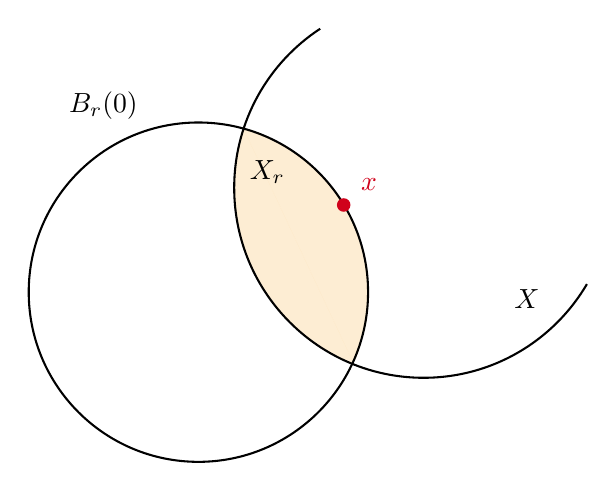
\begin{tikzpicture}[x=0.75pt,y=0.75pt,yscale=-1,xscale=1]
%uncomment if require: \path (0,230); %set diagram left start at 0, and has height of 230

%Curve Lines [id:da2504201730057849] 
\draw [color={rgb, 255:red, 0; green, 0; blue, 0 }  ,draw opacity=0 ][fill={rgb, 255:red, 245; green, 166; blue, 35 }  ,fill opacity=0.2 ]   (292.5,62) .. controls (275.5,114) and (307.5,162) .. (345.5,175) ;


%Curve Lines [id:da9282468110405973] 
\draw [color={rgb, 255:red, 0; green, 0; blue, 0 }  ,draw opacity=0 ][fill={rgb, 255:red, 245; green, 166; blue, 35 }  ,fill opacity=0.2 ]   (345.5,175) .. controls (361.5,140) and (351.5,80) .. (292.5,62) ;



%Shape: Arc [id:dp5893565110889671] 
\draw  [draw opacity=0] (457.94,136.85) .. controls (442.08,163.87) and (412.78,182) .. (379.25,182) .. controls (328.85,182) and (288,141.03) .. (288,90.5) .. controls (288,58.4) and (304.49,30.15) .. (329.44,13.82) -- (379.25,90.5) -- cycle ; \draw   (457.94,136.85) .. controls (442.08,163.87) and (412.78,182) .. (379.25,182) .. controls (328.85,182) and (288,141.03) .. (288,90.5) .. controls (288,58.4) and (304.49,30.15) .. (329.44,13.82) ;
%Shape: Circle [id:dp48240655002847554] 
\draw  [color={rgb, 255:red, 0; green, 0; blue, 0 }  ,draw opacity=1 ] (189,140.75) .. controls (189,95.6) and (225.6,59) .. (270.75,59) .. controls (315.9,59) and (352.5,95.6) .. (352.5,140.75) .. controls (352.5,185.9) and (315.9,222.5) .. (270.75,222.5) .. controls (225.6,222.5) and (189,185.9) .. (189,140.75) -- cycle ;
%Shape: Circle [id:dp47950031726927] 
\draw  [color={rgb, 255:red, 208; green, 2; blue, 27 }  ,draw opacity=1 ][fill={rgb, 255:red, 208; green, 2; blue, 27 }  ,fill opacity=1 ] (338,98.75) .. controls (338,97.23) and (339.23,96) .. (340.75,96) .. controls (342.27,96) and (343.5,97.23) .. (343.5,98.75) .. controls (343.5,100.27) and (342.27,101.5) .. (340.75,101.5) .. controls (339.23,101.5) and (338,100.27) .. (338,98.75) -- cycle ;

% Text Node
\draw (225,51) node [color={rgb, 255:red, 0; green, 0; blue, 0 }  ,opacity=1 ]  {$B_{r}( 0)$};
% Text Node
\draw (353,89) node [color={rgb, 255:red, 208; green, 2; blue, 27 }  ,opacity=1 ]  {$x$};
% Text Node
\draw (429,144) node   {$X$};
% Text Node
\draw (304,83) node [color={rgb, 255:red, 0; green, 0; blue, 0 }  ,opacity=1 ]  {$X_{r}$};


\end{tikzpicture}

		\end{center}
		\caption{Skizze von $X_{r}$}
		\label{fig:XR1}
	\end{figure}
	
\end{lemma}

\begin{proof}
%\label{thm:}
	\begin{itemize}
		\item "$\Longrightarrow$"
	
			Sei ${x}^{*}$ eine Lösung von VIP($X,F$). Dann gilt ${x}^{*} \in X_{r}$ und
			\[
				F({x}^{*})^{T}(x-{x}^{*}) \geq  0 \quad \forall x \in X \supseteq X_{r}
			.\] 
			$\implies {x}^{*}$ löst VIP($X,F$).
	
		\item "$\Longleftarrow$"
	
			Sei ${x}^{*} \in X_{r}$ eine Lösung von VIP($X_{r},F$). Dann gilt ${x}^{*} \in X$ und
			\[
				F({x}^{*})^{T}(x-{x}^{*}) \quad \forall x \in X \text{ mit } \norm{x}_{2}  \leq  r
			.\] 
			\begin{figure}[H]
				\begin{center}
					\tikzset{every picture/.style={line width=0.75pt}} %set default line width to 0.75pt        

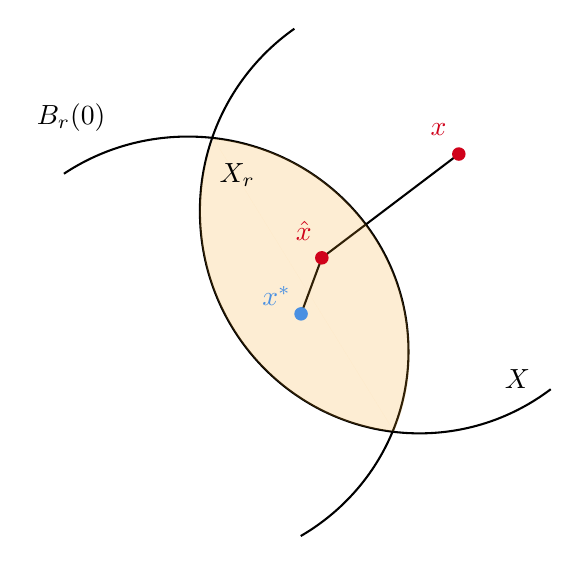
\begin{tikzpicture}[x=0.75pt,y=0.75pt,yscale=-1,xscale=1]
%uncomment if require: \path (0,269.33331298828125); %set diagram left start at 0, and has height of 269.33331298828125

%Straight Lines [id:da9081237263295667] 
\draw    (339.75,122.75) -- (405.75,72.75) ;


%Straight Lines [id:da013531378414466388] 
\draw    (329.75,149.75) -- (339.75,122.75) ;


%Shape: Arc [id:dp29762120971158423] 
\draw  [draw opacity=0] (450.04,186.06) .. controls (432.4,199.42) and (410.49,207.33) .. (386.75,207.33) .. controls (328.35,207.33) and (281,159.43) .. (281,100.33) .. controls (281,63.88) and (299.01,31.69) .. (326.52,12.37) -- (386.75,100.33) -- cycle ; \draw   (450.04,186.06) .. controls (432.4,199.42) and (410.49,207.33) .. (386.75,207.33) .. controls (328.35,207.33) and (281,159.43) .. (281,100.33) .. controls (281,63.88) and (299.01,31.69) .. (326.52,12.37) ;
%Shape: Arc [id:dp9736457048511031] 
\draw  [draw opacity=0] (215.51,82.23) .. controls (232.53,70.94) and (253.1,64.33) .. (275.25,64.33) .. controls (333.93,64.33) and (381.5,110.67) .. (381.5,167.83) .. controls (381.5,205.65) and (360.68,238.73) .. (329.59,256.79) -- (275.25,167.83) -- cycle ; \draw   (215.51,82.23) .. controls (232.53,70.94) and (253.1,64.33) .. (275.25,64.33) .. controls (333.93,64.33) and (381.5,110.67) .. (381.5,167.83) .. controls (381.5,205.65) and (360.68,238.73) .. (329.59,256.79) ;
%Curve Lines [id:da7464413291611462] 
\draw [color={rgb, 255:red, 0; green, 0; blue, 0 }  ,draw opacity=0 ][fill={rgb, 255:red, 245; green, 166; blue, 35 }  ,fill opacity=0.2 ]   (287.5,65.33) .. controls (262.5,132.33) and (312.5,201.33) .. (374.5,206.33) ;


%Curve Lines [id:da9820940956263626] 
\draw [color={rgb, 255:red, 0; green, 0; blue, 0 }  ,draw opacity=0 ][fill={rgb, 255:red, 245; green, 166; blue, 35 }  ,fill opacity=0.2 ]   (287.5,65.33) .. controls (360.5,72.33) and (399.5,149.33) .. (374.5,206.33) ;



%Shape: Circle [id:dp43139799952926605] 
\draw  [color={rgb, 255:red, 208; green, 2; blue, 27 }  ,draw opacity=1 ][fill={rgb, 255:red, 208; green, 2; blue, 27 }  ,fill opacity=1 ] (337,122.75) .. controls (337,121.23) and (338.23,120) .. (339.75,120) .. controls (341.27,120) and (342.5,121.23) .. (342.5,122.75) .. controls (342.5,124.27) and (341.27,125.5) .. (339.75,125.5) .. controls (338.23,125.5) and (337,124.27) .. (337,122.75) -- cycle ;
%Shape: Circle [id:dp14058981705181228] 
\draw  [color={rgb, 255:red, 208; green, 2; blue, 27 }  ,draw opacity=1 ][fill={rgb, 255:red, 208; green, 2; blue, 27 }  ,fill opacity=1 ] (403,72.75) .. controls (403,71.23) and (404.23,70) .. (405.75,70) .. controls (407.27,70) and (408.5,71.23) .. (408.5,72.75) .. controls (408.5,74.27) and (407.27,75.5) .. (405.75,75.5) .. controls (404.23,75.5) and (403,74.27) .. (403,72.75) -- cycle ;
%Shape: Circle [id:dp5811537747008597] 
\draw  [color={rgb, 255:red, 74; green, 144; blue, 226 }  ,draw opacity=1 ][fill={rgb, 255:red, 74; green, 144; blue, 226 }  ,fill opacity=1 ] (327,149.75) .. controls (327,148.23) and (328.23,147) .. (329.75,147) .. controls (331.27,147) and (332.5,148.23) .. (332.5,149.75) .. controls (332.5,151.27) and (331.27,152.5) .. (329.75,152.5) .. controls (328.23,152.5) and (327,151.27) .. (327,149.75) -- cycle ;


% Text Node
\draw (434,181) node   {$X$};
% Text Node
\draw (219,55) node   {$B_{r}( 0)$};
% Text Node
\draw (299,83) node   {$X_{r}$};
% Text Node
\draw (396,61) node [color={rgb, 255:red, 208; green, 2; blue, 27 }  ,opacity=1 ]  {$x$};
% Text Node
\draw (331,110) node [color={rgb, 255:red, 208; green, 2; blue, 27 }  ,opacity=1 ]  {$\hat{x}$};
% Text Node
\draw (318,141) node [color={rgb, 255:red, 74; green, 144; blue, 226 }  ,opacity=1 ]  {$x^{*}$};
\end{tikzpicture}

				\end{center}
				\caption{Skizze von Definition von $\hat{x}$}
				\label{fig:XR2}
			\end{figure}
			
			Sei $x \in X \setminus  X_{r}$ beliebig. Dann gilt wegen $\norm{{x}^{*}}_{2}< r$
			\[
				\hat{x} = {x}^{*} + c(x-{x}^{*}) \quad \text{ für }c>0 \text{ klein } \hat{x} \in X_{r}
			.\] 
			Also
			\begin{align*}
				&\implies F({x}^{*})^{T}(\hat{x}-{x}^{*}) = F({x}^{*})^{T}({x}^{*} + c (x-{x}^{*}) - {x}^{*}) \geq  0 \\
				&\implies F({x}^{*})^{T}(x-{x}^{*}) \geq  0
			\end{align*}
			
	\end{itemize}
	
\end{proof}

\begin{satz}
%\label{thm:}
	Sei
	\begin{itemize}
		\item $X \subseteq \R^{n}$ nichtleer, abgeschlossen, konvex
		\item $F \colon X \rightarrow \R^{n} $ stetig
	\end{itemize}
	Gibt es einen Punkt $\overline{x} \in X$ mit
	\[
		\lim_{\substack{\norm{x}_{2} \rightarrow \infty \\ x \in X}} \frac{(F(x) - F(\overline{x}))^{T}(x-\overline{x})}{\norm{x-\overline{x}}_{2} } = + \infty
	\] 
	dann hat das VIP($X,F$) mindestens eine Lösung.
\end{satz}

\begin{figure}[H]
	\begin{center}
		\tikzset{every picture/.style={line width=0.75pt}} %set default line width to 0.75pt        

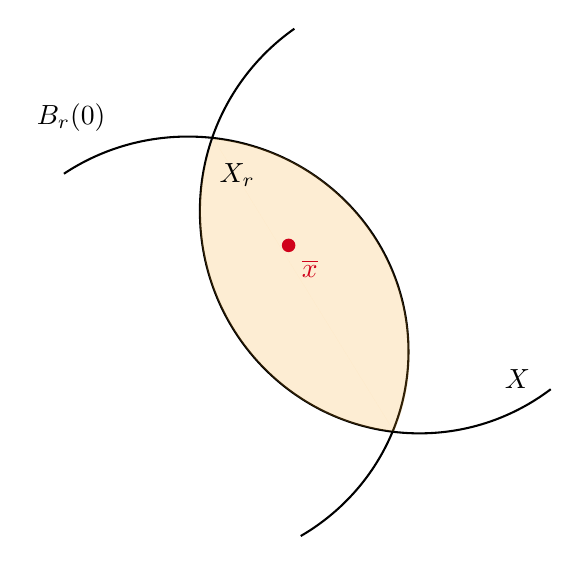
\begin{tikzpicture}[x=0.75pt,y=0.75pt,yscale=-1,xscale=1]
%uncomment if require: \path (0,264.34375); %set diagram left start at 0, and has height of 264.34375

%Shape: Arc [id:dp8108185124259488] 
\draw  [draw opacity=0] (450.04,184.06) .. controls (432.4,197.42) and (410.49,205.33) .. (386.75,205.33) .. controls (328.35,205.33) and (281,157.43) .. (281,98.33) .. controls (281,61.88) and (299.01,29.69) .. (326.52,10.37) -- (386.75,98.33) -- cycle ; \draw   (450.04,184.06) .. controls (432.4,197.42) and (410.49,205.33) .. (386.75,205.33) .. controls (328.35,205.33) and (281,157.43) .. (281,98.33) .. controls (281,61.88) and (299.01,29.69) .. (326.52,10.37) ;
%Shape: Arc [id:dp37084419859759254] 
\draw  [draw opacity=0] (215.51,80.23) .. controls (232.53,68.94) and (253.1,62.33) .. (275.25,62.33) .. controls (333.93,62.33) and (381.5,108.67) .. (381.5,165.83) .. controls (381.5,203.65) and (360.68,236.73) .. (329.59,254.79) -- (275.25,165.83) -- cycle ; \draw   (215.51,80.23) .. controls (232.53,68.94) and (253.1,62.33) .. (275.25,62.33) .. controls (333.93,62.33) and (381.5,108.67) .. (381.5,165.83) .. controls (381.5,203.65) and (360.68,236.73) .. (329.59,254.79) ;
%Curve Lines [id:da8089221113106915] 
\draw [color={rgb, 255:red, 0; green, 0; blue, 0 }  ,draw opacity=0 ][fill={rgb, 255:red, 245; green, 166; blue, 35 }  ,fill opacity=0.2 ]   (287.5,63.33) .. controls (262.5,130.33) and (312.5,199.33) .. (374.5,204.33) ;


%Curve Lines [id:da5363406730646809] 
\draw [color={rgb, 255:red, 0; green, 0; blue, 0 }  ,draw opacity=0 ][fill={rgb, 255:red, 245; green, 166; blue, 35 }  ,fill opacity=0.2 ]   (287.5,63.33) .. controls (360.5,70.33) and (399.5,147.33) .. (374.5,204.33) ;



%Shape: Circle [id:dp5519419662089802] 
\draw  [color={rgb, 255:red, 208; green, 2; blue, 27 }  ,draw opacity=1 ][fill={rgb, 255:red, 208; green, 2; blue, 27 }  ,fill opacity=1 ] (321,114.75) .. controls (321,113.23) and (322.23,112) .. (323.75,112) .. controls (325.27,112) and (326.5,113.23) .. (326.5,114.75) .. controls (326.5,116.27) and (325.27,117.5) .. (323.75,117.5) .. controls (322.23,117.5) and (321,116.27) .. (321,114.75) -- cycle ;

% Text Node
\draw (434,179) node   {$X$};
% Text Node
\draw (219,53) node   {$B_{r}( 0)$};
% Text Node
\draw (299,81) node   {$X_{r}$};
% Text Node
\draw (334,126) node [color={rgb, 255:red, 208; green, 2; blue, 27 }  ,opacity=1 ]  {$\overline{x}$};


\end{tikzpicture}

	\end{center}
	\caption{Skizze von $\overline{x}$}
	\label{fig:XR3}
\end{figure}
	
\begin{proof}
	Wähle $r > \norm{\overline{x}}_{2} $ und $\mu > \norm{F(\overline{x})} _{2}$ mit
	\[
		\Big( F(x) - F(\overline{x}) \Big) ^{T}(x-\overline{x}) \geq  \mu  \norm{x -\overline{x}} _{2} \qquad \forall x \in X \text{ mit } \norm{x} _{2} \geq  r
	.\] 
	Daraus folgt für alle $x \in X$ mit $\norm{x} _{2}\geq r$ gilt
	\[
		F(x)^{T}(x-\overline{x}) \geq  \mu \norm{x-\overline{x}} - \underbrace{F(\overline{x})^{T}(x-\overline{x})}_{\leq \norm{F(\overline{x})} _{2}\norm{x-\overline{x}} _{2}} \geq \underbrace{(\mu -\norm{F(\overline{x})} _{2})}_{>0} \underbrace{\norm{x-\overline{x}} _{2}}_{>0} >0
	.\] 
	Daraus folgt wiederum, dass das VIP($X,F$) keine Lösung haben kann mit $\norm{{x}^{*}} _{2}\geq  r$.

	Da $X_{r}$ nichtleer, konvex, kompakt \& $F$ stetig ist, gibt es eine Lösung ${x}^{*}$ von VIP($X_{r},F$).

	Aus $\overline{x} \in X_{r}$ folgt
	\[
		F({x}^{*})^{T}(\overline{x}-{x}^{*})\geq 0 \implies \norm{{x}^{*}} _{2}< r
	.\] 
	Mit dem Lemma folgt, dass ${x}^{*}$ eine Lösung von VIP($X,F$) ist.
\end{proof}
